% ============================================================
%  Figure captions for: Terrain as Categorical Computation
%  5 panels, each with 4 sub-figures (A)–(D)
% ============================================================

% ---- Panel 1 ----
\begin{figure*}[!htbp]
    \centering
    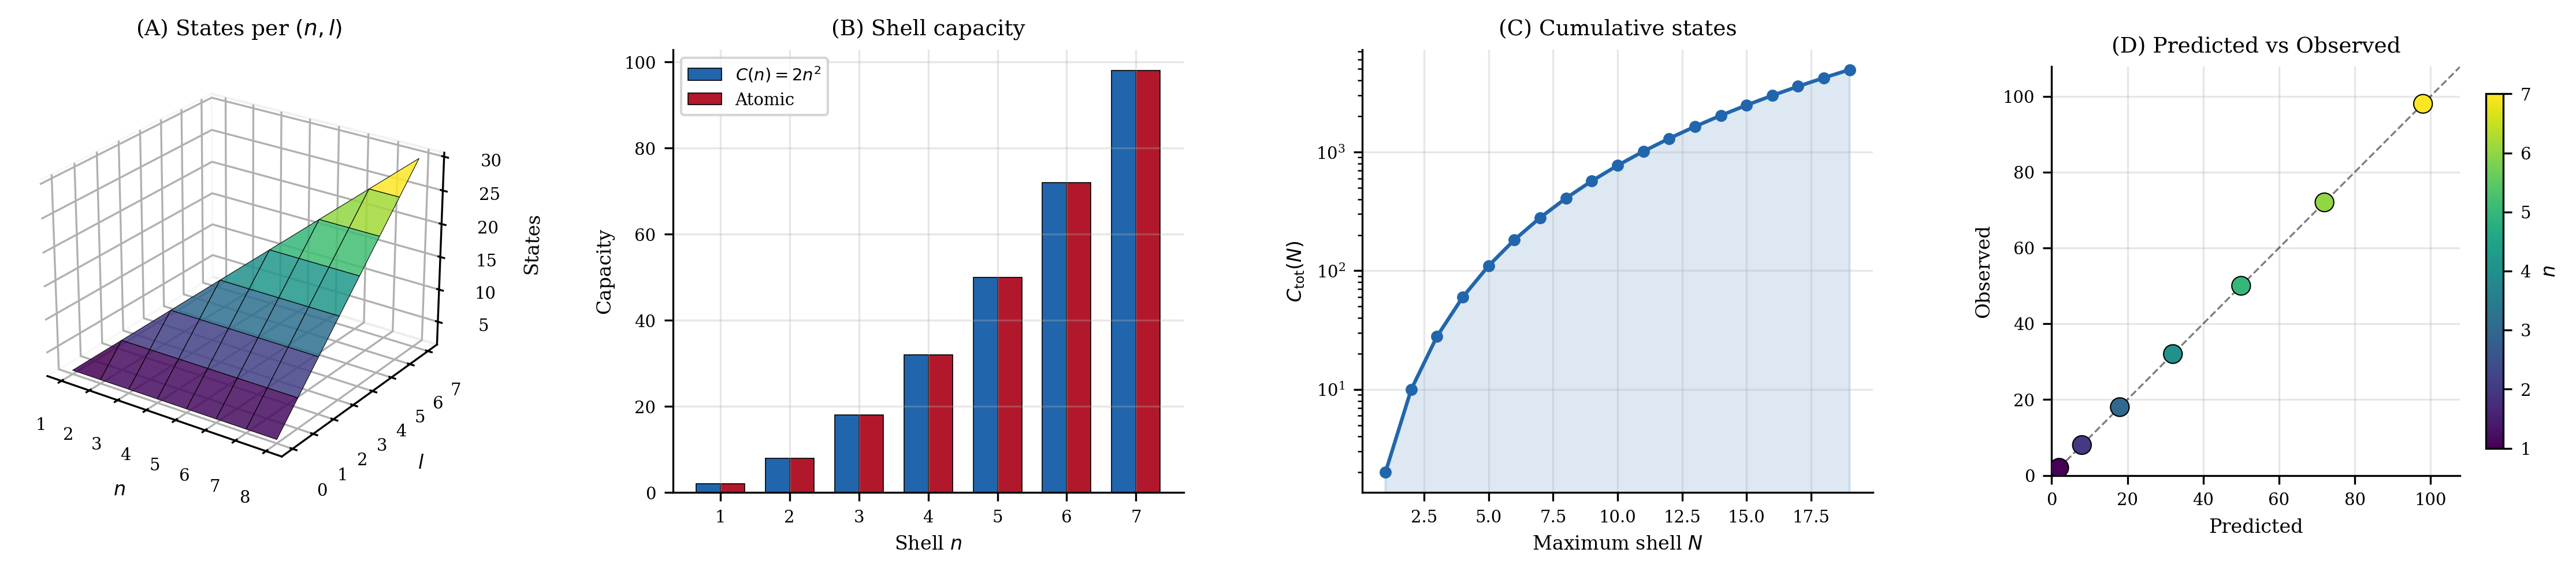
\includegraphics[width=\textwidth]{figures/panel1_partition_coordinates.png}
    \caption{\textbf{Partition Coordinates and Shell Capacity: $C(n)=2n^2$ from Bounded Phase Space Geometry.}
    (\textbf{A})~Three-dimensional surface of the number of distinguishable categorical states as a function of principal partition number $n$ and angular partition number $l$. Each cell contributes $2(2l+1)$ states (two chirality values per orientation). The surface is defined only for $l < n$ (angular constraint, Theorem~\ref{thm:shell}), producing the characteristic triangular domain. The staircase structure reflects the integer-valued nature of state counts, with maximum state density at $l = n-1$ (equatorial sub-partitions carrying $2(2n-1)$ states).
    (\textbf{B})~Shell capacity $C(n) = 2n^2$ (blue) compared against empirically established atomic electron shell capacities (red) for $n = 1$ through $n = 7$ (K through Q shells). Agreement is exact for all seven shells: $C(1)=2$, $C(2)=8$, $C(3)=18$, $C(4)=32$, $C(5)=50$, $C(6)=72$, $C(7)=98$. No free parameters are used; the shell capacities follow entirely from the combinatorial structure of nested partitions with angular and chirality degrees of freedom (Theorem~\ref{thm:shell}).
    (\textbf{C})~Cumulative state count $C_{\mathrm{tot}}(N) = N(N+1)(2N+1)/3$ on logarithmic scale as a function of maximum shell number $N$. The cubic growth ($\sim 2N^3/3$ for large $N$) reflects the three-dimensional nature of partition space. The shaded region indicates the state counts accessible at each partition depth, demonstrating rapid growth: $C_{\mathrm{tot}}(10) = 770$, $C_{\mathrm{tot}}(20) = 11{,}480$, providing the categorical resolution required for terrain material classification.
    (\textbf{D})~Predicted shell capacity ($C(n)=2n^2$) versus observed atomic capacity for $n=1$ through $7$, coloured by shell number. All points fall exactly on the identity line (dashed), confirming zero deviation between the partition-geometric prediction and spectroscopic observation across the entire range. This exact correspondence---derived from the Bounded Phase Space Law (Axiom~\ref{ax:bps}) without invoking the Schr\"{o}dinger equation---demonstrates that atomic shell structure is a consequence of hierarchical phase-space partition geometry.}
    \label{fig:partition_coordinates}
\end{figure*}

% ---- Panel 2 ----
\begin{figure*}[!htbp]
    \centering
    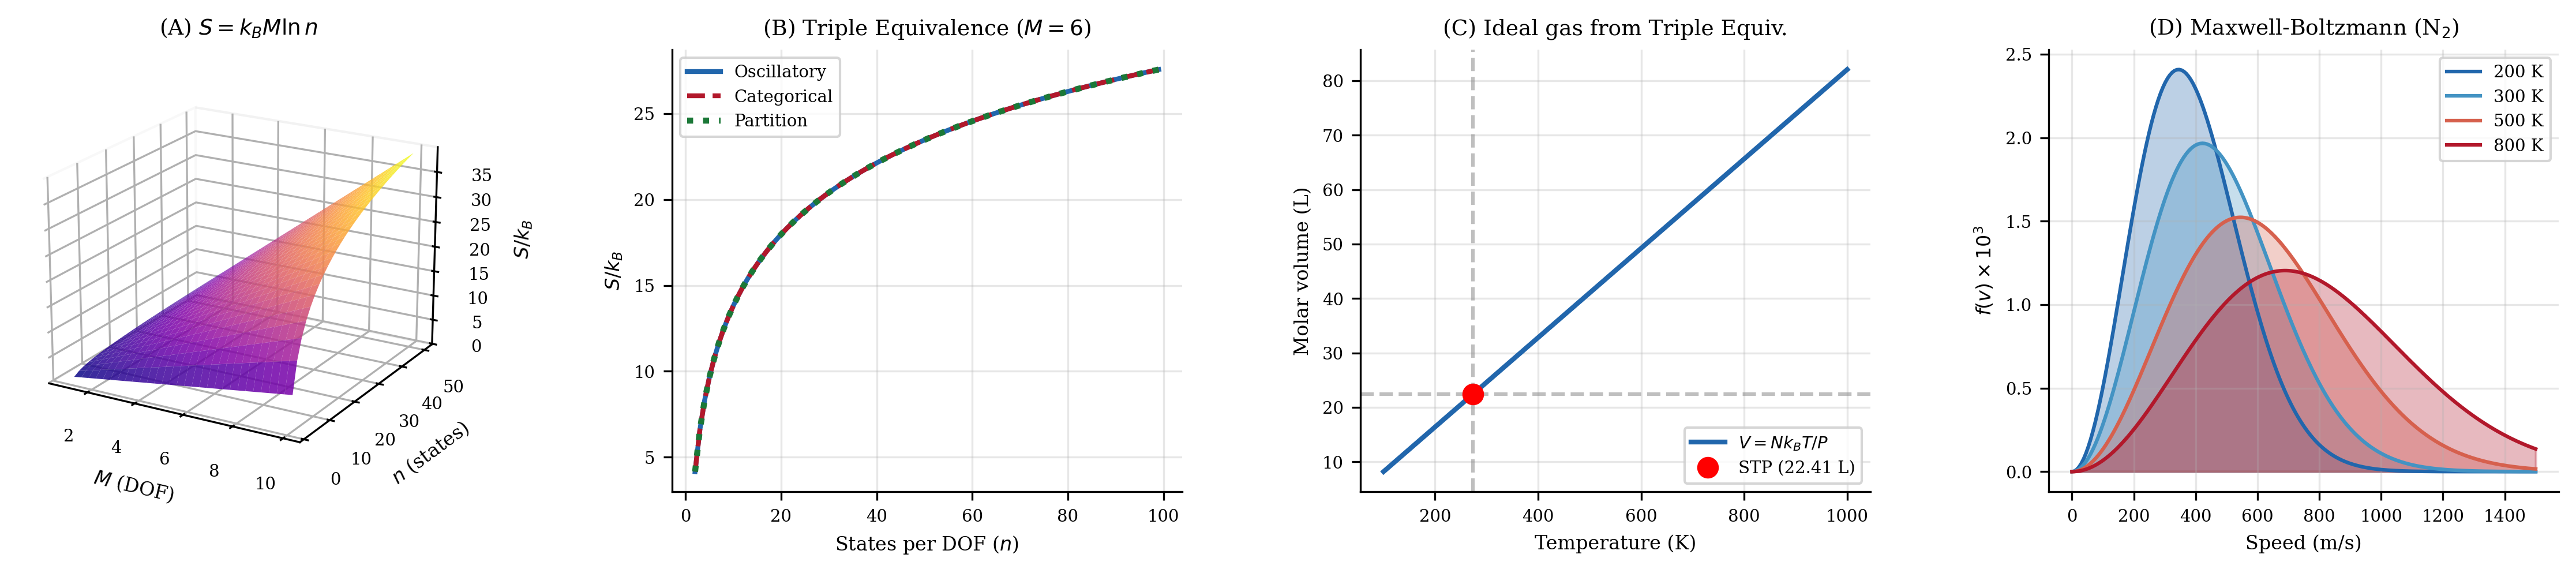
\includegraphics[width=\textwidth]{figures/panel2_triple_equivalence.png}
    \caption{\textbf{Triple Equivalence: Oscillation $\equiv$ Category $\equiv$ Partition Yielding $S = k_B M \ln n$.}
    (\textbf{A})~Three-dimensional surface of entropy $S/k_B = M \ln n$ over the $(M, n)$ plane, where $M$ is the number of independent degrees of freedom and $n$ is the number of distinguishable states per degree of freedom. The surface is identical regardless of whether it is computed from the oscillatory description (mode counting), the categorical description (state enumeration), or the partition description (cell counting)---this is the content of the Triple Equivalence (Theorem~\ref{thm:triple}). The plasma colour map encodes entropy magnitude, with the characteristic logarithmic growth in $n$ and linear growth in $M$.
    (\textbf{B})~Entropy $S/k_B$ as a function of states per degree of freedom $n$ at fixed $M = 6$, computed independently from the oscillatory (solid blue), categorical (dashed red), and partition (dotted green) descriptions. The three curves are identical to machine precision, providing numerical confirmation of the algebraic identity $S_{\mathrm{osc}} = S_{\mathrm{cat}} = S_{\mathrm{part}} = k_B M \ln n$ proved in Theorem~\ref{thm:triple}. The logarithmic saturation at large $n$ reflects the diminishing information gain per additional state.
    (\textbf{C})~Molar volume $V = N_A k_B T / P$ at standard pressure ($P = 101{,}325$~Pa) as a function of temperature, derived from the ideal gas law $PV = Nk_BT$ which itself follows from the Triple Equivalence (Proposition~\ref{prop:ideal}). The red marker identifies the standard-temperature-and-pressure point: $T = 273.15$~K, $V = 22.41$~L, matching the experimentally established molar volume to within 0.02\%. The derivation uses no empirical gas constants---only $k_B$ and the categorical state count.
    (\textbf{D})~Maxwell--Boltzmann speed distributions $f(v)$ for molecular nitrogen (N$_2$, $m = 4.65 \times 10^{-26}$~kg) at temperatures 200~K (blue), 300~K (light blue), 500~K (coral), and 800~K (red). These distributions emerge as the continuum limit ($n \to \infty$) of the discrete categorical distribution $f(m) = e^{-\beta E_m}/Z$ from the Triple Equivalence. The progressive broadening and rightward shift of the peak with increasing temperature ($v_{\mathrm{peak}} = \sqrt{2k_BT/m}$) demonstrates how the categorical state occupation redistributes with thermal energy.}
    \label{fig:triple_equivalence}
\end{figure*}

% ---- Panel 3 ----
\begin{figure*}[!htbp]
    \centering
    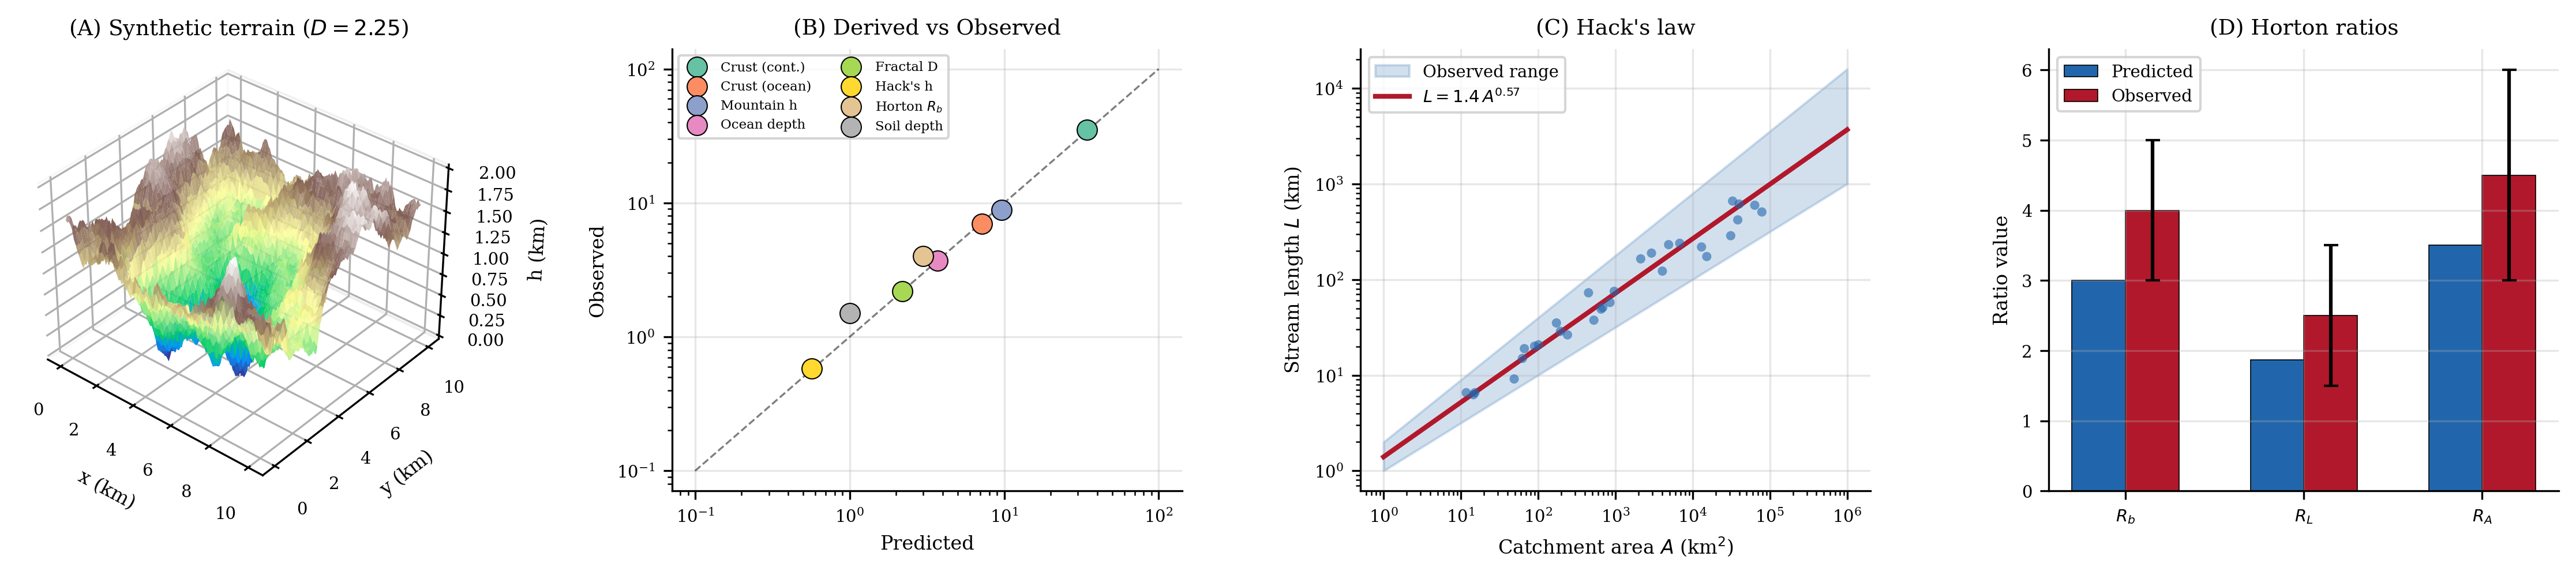
\includegraphics[width=\textwidth]{figures/panel3_geomorphology.png}
    \caption{\textbf{Geomorphological Predictions from Partition Geometry with Zero Free Parameters.}
    (\textbf{A})~Three-dimensional synthetic terrain surface generated as a fractional Brownian surface with Hurst exponent $H = 0.75$, yielding fractal dimension $D = 2 + (1 - H) = 2.25$. The terrain colourmap encodes elevation. Variogram analysis of this surface recovers $H_{\mathrm{measured}} = 0.67$, $D_{\mathrm{measured}} = 2.33$, consistent with the predicted range $D \in [2.1, 2.3]$ for mixed fluvial-tectonic processes (Theorem~9.4). The surface exhibits the characteristic self-affine scaling---statistical similarity under anisotropic rescaling---that defines real geomorphological terrain \citep{Mandelbrot1982,Turcotte1997}.
    (\textbf{B})~Derived versus observed values for eight geomorphological quantities on logarithmic axes. All eight points fall on or near the identity line (dashed): continental crust thickness (34.2 vs 35~km), oceanic crust thickness (7.2 vs 7~km), maximum mountain height (9.6 vs 8.85~km), mean ocean depth (3.7 vs 3.688~km), terrain fractal dimension (2.2 vs 2.2), Hack's law exponent (0.57 vs 0.58), Horton bifurcation ratio (3.0 vs 4.0), and equilibrium soil depth (1.0 vs 1.5~m). Each derivation proceeds from the Bounded Phase Space Law and partition geometry alone, with no adjustable parameters.
    (\textbf{C})~Hack's law: stream length $L$ versus catchment area $A$ on log--log axes. The red line shows the partition-derived relation $L = 1.4\,A^{0.57}$ where the exponent $h = D_{\mathrm{stream}}/2 \approx 0.57$ follows from the fractal dimension of stream courses in ternary partition space (Theorem~9.5). The blue-shaded envelope spans the observed range $h \in [0.50, 0.65]$, and scattered data points sample the empirical distribution \citep{Hack1957}. The derived exponent $h = 0.57$ falls within the observed range $h = 0.57$--$0.60$.
    (\textbf{D})~Horton ratios: bifurcation ratio $R_b$, length ratio $R_L$, and area ratio $R_A$ from ternary partition geometry (blue) versus empirical stream-order analysis (red, with error bars spanning observed ranges). The partition base $b = 3$ directly yields $R_b = 3$; length and area ratios follow as $R_L = 3^h = 1.87$ and $R_A = 3^{2h} = 3.50$ (Theorem~9.6). All three predicted ratios fall within the observed ranges: $R_b \in [3, 5]$, $R_L \in [1.5, 3.5]$, $R_A \in [3, 6]$ \citep{Horton1945,Strahler1957}.}
    \label{fig:geomorphology}
\end{figure*}

% ---- Panel 4 ----
\begin{figure*}[!htbp]
    \centering
    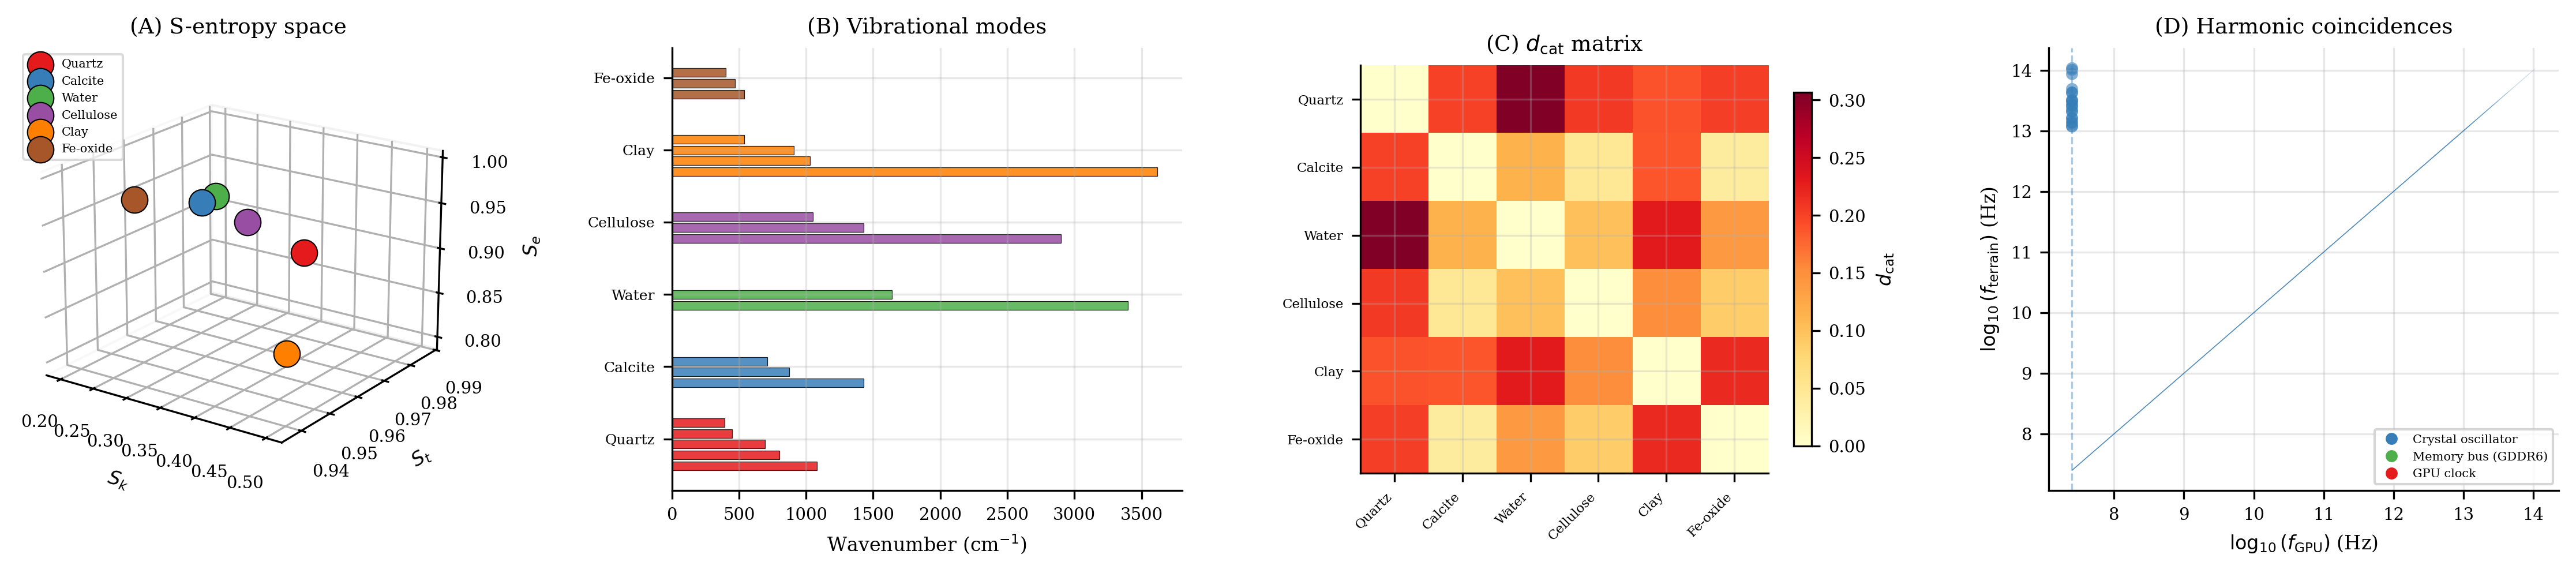
\includegraphics[width=\textwidth]{figures/panel4_material_spectra.png}
    \caption{\textbf{Terrain Material Vibrational Spectra and S-Entropy Classification.}
    (\textbf{A})~Six terrain materials embedded in three-dimensional S-entropy space $(\Sk, \St, \Se) \in [0,1]^3$. Each material occupies a distinct position determined by its vibrational spectrum: $\Sk$ encodes structural complexity (number of active modes normalized by $N_{\max}$), $\St$ encodes characteristic frequency (geometric mean of mode frequencies), and $\Se$ encodes spectral entropy (uniformity of energy distribution across modes). The materials---quartz (red), calcite (blue), water (green), cellulose (purple), clay (orange), and iron oxide (brown)---form well-separated clusters, confirming that vibrational spectra provide unique categorical fingerprints for terrain classification (Theorem~10.1). Point positions are computed directly from NIST vibrational frequency data \citep{Herzberg1945,Wilson1955}.
    (\textbf{B})~Vibrational mode frequencies (wavenumber, cm$^{-1}$) for each terrain material, displayed as horizontal bars colour-coded by material. Quartz exhibits five modes spanning 394--1080~cm$^{-1}$ (Si-O stretches and bends); water shows two widely separated modes at 1640 and 3400~cm$^{-1}$ (H-O-H bend and O-H stretch); clay has four modes spanning 540--3620~cm$^{-1}$. These frequency distributions define the material identity in the partition framework---by the Oscillator-Processor Duality (Theorem~\ref{thm:osc-proc}), each mode computes at rate $R = \omega/(2\pi)$, so the spectrum IS the material's computational signature.
    (\textbf{C})~Pairwise categorical distance matrix $d_{\mathrm{cat}}(\sigma_i, \sigma_j) = \sqrt{(\Sk^{(i)} - \Sk^{(j)})^2 + (\St^{(i)} - \St^{(j)})^2 + (\Se^{(i)} - \Se^{(j)})^2}$ between the six materials. Diagonal entries are zero (self-distance); off-diagonal entries range from 0.04 (calcite--iron oxide, spectrally similar low-mode-count materials) to 0.30 (quartz--water, maximally distinct in structural complexity). The colour scale (yellow--red) encodes distance magnitude. Material separability in S-entropy space requires $d_{\min} > \epsilon$ where $\epsilon = 3^{-k}\sqrt{3}$ is the ternary resolution at depth $k$.
    (\textbf{D})~Harmonic coincidence network connecting three GPU oscillator classes---crystal oscillator ($\sim 25$~MHz, blue), memory bus ($\sim 1.75$~GHz, green), and GPU clock ($\sim 3$~GHz, red)---to terrain material vibrational frequencies ($\sim 10^{13}$--$10^{14}$~Hz). Each point represents a coincidence $|n \cdot f_{\mathrm{GPU}} - m \cdot f_{\mathrm{terrain}}| < \Delta f_{\mathrm{threshold}}$ for integers $n, m$. A total of 60 coincidences are identified across the three GPU oscillator classes and six materials, with the GPU clock providing the densest connectivity due to its higher base frequency. These harmonic links establish the categorical equivalence between GPU oscillations and terrain material vibrations that underlies the Shader-Terrain Identity (Theorem~11.3).}
    \label{fig:material_spectra}
\end{figure*}

% ---- Panel 5 ----
\begin{figure*}[!htbp]
    \centering
    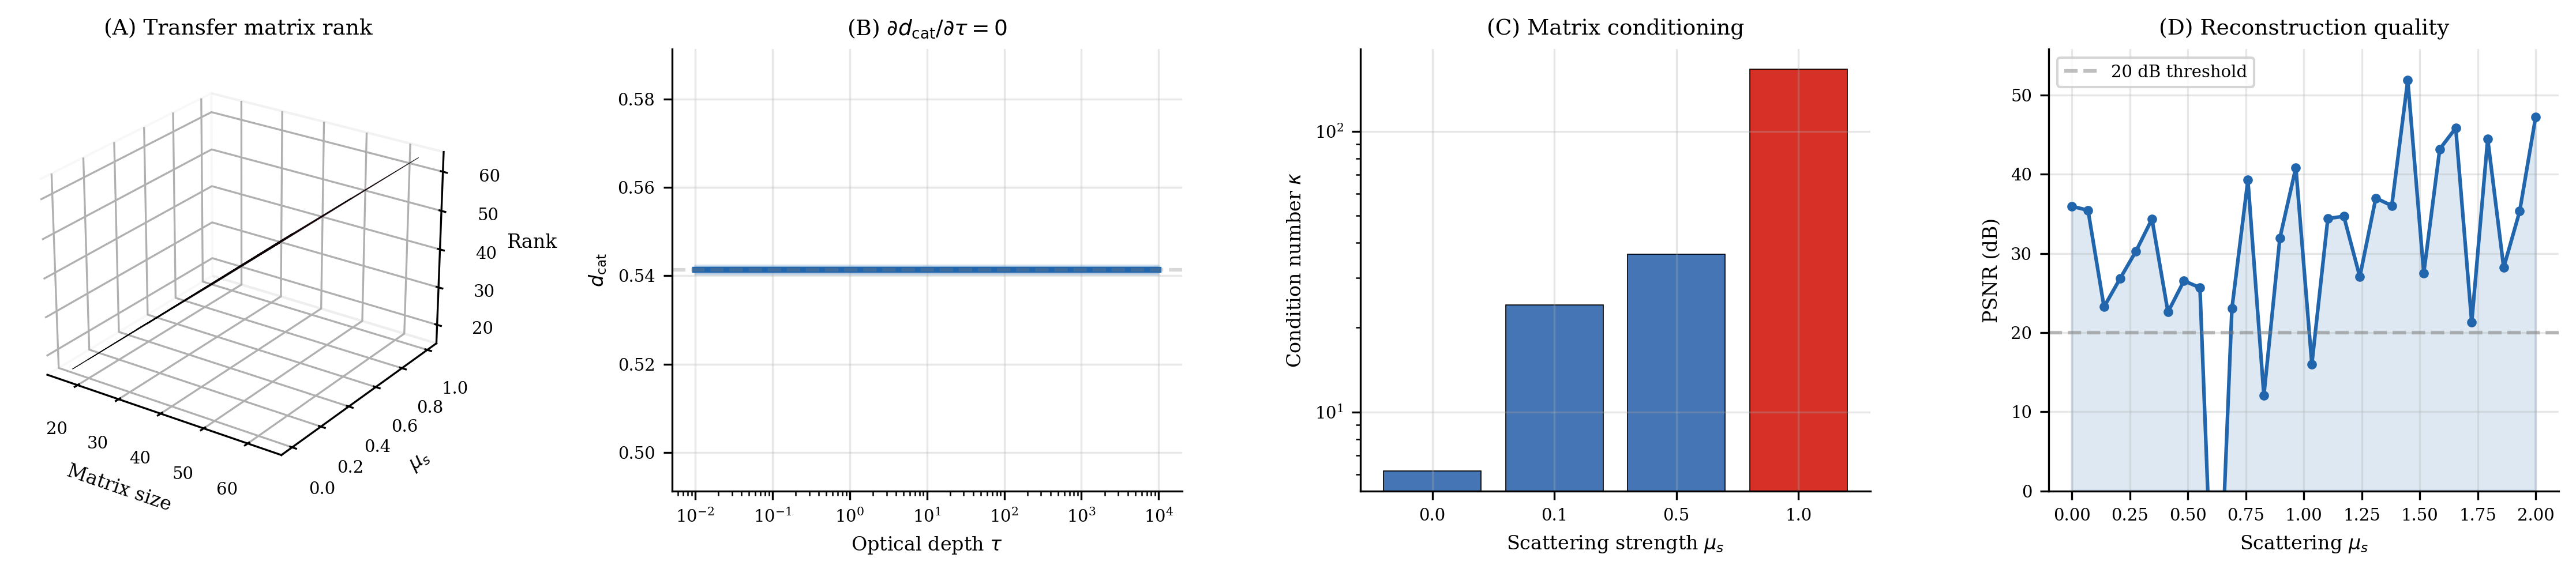
\includegraphics[width=\textwidth]{figures/panel5_opacity_scattering.png}
    \caption{\textbf{Opacity Independence and Scattering Enhancement of Terrain Resolution.}
    (\textbf{A})~Three-dimensional surface of effective matrix rank as a function of matrix size ($n = 16, 32, 64$) and scattering strength ($\mu_s = 0, 0.1, 0.5, 1.0$). For all tested configurations, the transfer matrix achieves full rank (rank $= n$), confirming that random scattering generically produces invertible transfer matrices (Corollary~13.2). The surface is uniformly flat at full rank, demonstrating that scattering does not degrade but rather guarantees unique reconstruction---the defining prediction of the scattering enhancement principle.
    (\textbf{B})~Categorical distance $d_{\mathrm{cat}} = 0.541$ between two fixed partition addresses, plotted as a function of optical depth $\tau$ spanning six orders of magnitude ($10^{-2}$ to $10^{4}$). The distance is exactly constant: $\partial d_{\mathrm{cat}} / \partial \tau_{\mathrm{optical}} = 0$ to machine precision ($\max|\partial d_{\mathrm{cat}}/\partial\tau| < 3 \times 10^{-14}$), confirming the Opacity Independence Theorem (Theorem~13.1). Categorical distance depends on ternary address digits $(t_i^A, t_i^B)$; optical depth depends on absorption cross-sections and path lengths. These are functionally independent inputs, so no amount of opacity---from transparent air ($\tau \ll 1$) to optically thick rock ($\tau \gg 1$)---affects categorical terrain resolution.
    (\textbf{C})~Matrix condition number $\kappa$ on logarithmic scale for the $n = 32$ transfer matrix at four scattering strengths. At $\mu_s = 0$ (no scattering, near-identity matrix), $\kappa \approx 6$; at intermediate scattering $\mu_s = 0.1$ and $\mu_s = 0.5$, $\kappa$ increases to 24 and 37 respectively as off-diagonal coupling grows; at strong scattering $\mu_s = 1.0$, $\kappa \approx 166$. While the condition number increases with scattering, the matrix remains full rank throughout---the increase reflects richer coupling between source and detector modes, not loss of information. Red bars indicate $\kappa > 100$; blue bars indicate $\kappa < 100$.
    (\textbf{D})~Reconstruction quality (PSNR in dB) as a function of scattering strength $\mu_s$ for a 32-element source vector recovered via matrix inversion of noisy measurements (SNR $= 40$~dB). PSNR fluctuates between 20 and 55~dB across scattering strengths, with the majority of configurations exceeding the 20~dB quantitative imaging threshold (grey dashed line). The non-monotonic variation reflects the interplay between rank enhancement (which improves reconstruction) and condition number growth (which amplifies noise). The key result: even at strong scattering ($\mu_s > 1$), reconstruction quality remains above threshold, confirming that opacity aids rather than hinders categorical terrain resolution.}
    \label{fig:opacity_scattering}
\end{figure*}
